%%%%%%%%%%%%%%%%%%%%%%%%%%%%%%%%%%%%%%%%%%%%%%
%% Created by John Paul Minda, PhD			%%
%% Professor of Psychology					%%
%% The Brain and Mind Institute				%%
%% The University of Western Ontario		%%	
%% London, ON N6A 5C2						%%
%%											%%
%% Version 1.2								%%	
%% Feb 13, 2018								%%
%%%%%%%%%%%%%%%%%%%%%%%%%%%%%%%%%%%%%%%%%%%%%%

\documentclass{article}

\usepackage{fullpage}
\usepackage[brazilian]{babel}
\usepackage[utf8]{inputenc}
\usepackage[T1]{fontenc}

\usepackage[a5paper]{geometry}
\renewcommand{\familydefault}{\sfdefault}
\usepackage[scaled=1]{helvet}
\usepackage[helvet]{sfmath}
\everymath={\sf}
\usepackage{pdflscape}
\usepackage{rotating}

\usepackage{tikz}
\usetikzlibrary{calc}

\usepackage{graphicx}
\graphicspath{{./images/}}

\usepackage{parskip}
\usepackage[colorinlistoftodos]{todonotes}
\usepackage[colorlinks=true, allcolors=blue]{hyperref}

\title{Manual Do Calouro}
\author{Calico - Centro Acadêmico Livre da Computação}
\setcounter{tocdepth}{2}

\begin{document}


% Capa
\newgeometry{margin=0em,top=0em}
    \vspace{5cm}
    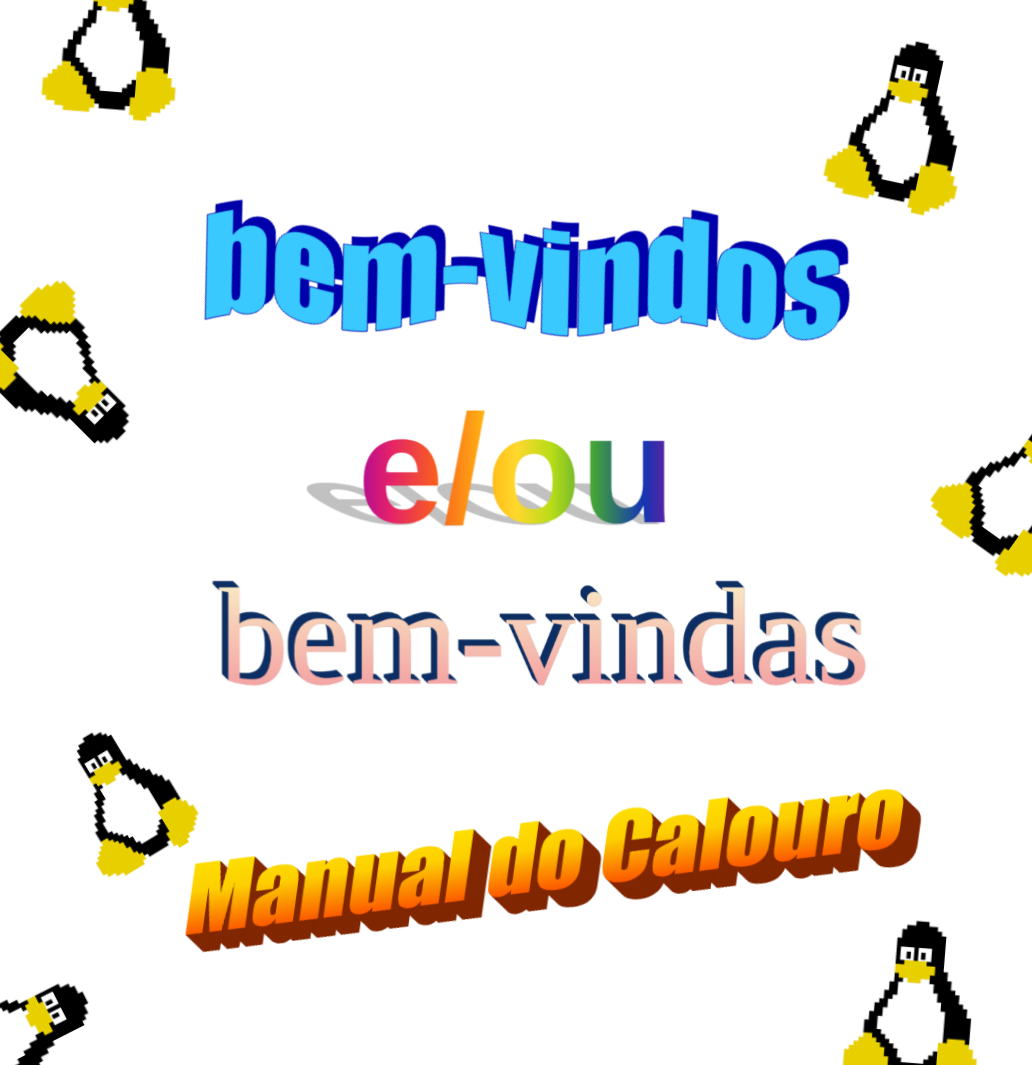
\includegraphics[width=\paperwidth,height=\paperheight]{capa}
\restoregeometry
% /Capa

\maketitle
\tableofcontents

\clearpage

\section{Entidades} 
Cada curso possui um Centro Acadêmico, sendo este uma instituição formada por alunos com o qual os estudantes se reúnem regularmente para discutir a situação do curso, de toda a universidade (ou mesmo de fora dela) e organizar atividades. São as entidades com maior potencial para identificar as demandas locais e articular entre alunas e alunos do curso, a fim de que possam conquistar suas reivindicações.
Ao Calico são atribuídas diversas funções, dentre elas:
\begin{itemize}
\item Auxiliar graduandos com problemas acadêmicos.
\item Representar os alunos do curso na esfera política da universidade, além de defender os interesses dos graduandos perante a Coordenação do curso.
\item Facilitar a socialização dos alunos, seja através de eventos de integração ou seja ocupando o espaço físico do calico.
\end{itemize}
 
O Calico se localiza subindo as escadas ao lado do Bar do CTC, no CETEC, onde são mantidas todas as salas de centros acadêmicos do CTC. A presença de todos é mais que bem-vinda para tomar café, estudar, conversar ou jogar PS4 :)
\subsubsection{Canais e mídias sociais}
Para ficar ligado e saber quando vão ocorrer os eventos ou pra ficar por dentro do que tá rolando na computação e na UFSC, siga nosso instagram @calicoufsc e se inscreva nos nossos canais de notícias no Telegram (@noticiascalico) ou Whatsapp (peça para um de nossos representantes te colocar)!

A gestão de 2019 (Gestão Turing) é composta por vários membros, sendo algum deles:
\begin{itemize}
\item Presidente: Caio Oliveira (@caiopo)
\item Vice-Presidente: Patrick Machado (@patrickmcds)
\item Tesoureiro: Cauê Baasch (@cauebs)
\item Secretário Geral: João Gabriel Trombeta (@gabrieltron)
\item Secretária Executiva: Paloma Cione (@zankely)
\end{itemize}
\subsection{DCE}
Além dos Centros Acadêmicos, existe o Diretório Central dos Estudantes, que engloba os estudantes de todos os campi da UFSC. O DCE é um dos principais instrumentos de luta dos
alunos e alunas, capaz de articular e orientar as reivindicações que dizem respeito a toda a
comunidade universitária. A partir dele, estudantes podem reconhecer que há problemas em
comum entre os centros, identificar possíveis soluções a partir de exemplos já aplicados em
outras localidades e desenvolver conjuntamente o melhor projeto para a UFSC no âmbito de
toda sua comunidade.

\subsection{PET}
O PET (Programa de Extensão Tutorial) foi criado pelo MEC e tem como objetivo principal desenvolver ações que promovam uma formação ampla e de qualidade aos estudantes envolvidos direta ou indiretamente com o programa, através de atividades de ensino, pesquisa e extensão.

Sendo composto por bolsistas participantes, sob a orientação de um professor tutor e atuação coletiva, ele promove condições para a realização de atividades extracurriculares, que favoreçam sua formação acadêmica global, contribuindo para a integração no mercado profissional, como também para o envolvimento no desenvolvimento de estudos em programas de Pós-Graduação. Outro grande objetivo do PET é a contribuição para a melhoria do ensino de graduação.
Você pode comparecer ao PET (sala 521, INE, quinto andar) para estudar, tirar dúvidas e participar ativamente dos projetos que ocorrem.

\subsection{Caravela Hacker Club}
O Caravela HackerClub é uma entidade que promove o desenvolvimento aberto e colaborativo de conhecimento e tecnologia. Organiza eventos e oferece minicursos e workshops para troca de experiência. Se você tem interesse em aprender ou ensinar sobre software ou hardware, faça uma visita à sala 418 do INE. Também estão sempre dispostos a ajudar no grupo no Telegram, em @CaravelaHC.

\subsection{Pixel}
A Pixel é a empresa júnior (EJ) dos cursos de Sistemas de Informação e Ciência da Computação que, atualmente, trabalha com o desenvolvimento de sites e e-commerce. As empresas juniores são iniciativas estudantis que promovem, por meio da atividade econômica, a vivência empresarial dentro da universidade. São projetos de extensão que, com orientação dos professores da universidade, realizam consultorias, projetos e serviços a pequenas empresas e microempreendedores individuais a preços reduzidos. Não tenha medo, calouro! Não é exigido nenhum tipo de experiência para trabalhar na Pixel. Grande parte da equipe atual entrou logo na primeira fase, e todos passaram por um processo de treinamento em que todo conhecimento básico necessário foi ensinado.

Conheça mais sobre a Pixel em \url{pixel.ufsc.br} e sobre o Movimento Empresa Júnior em \url{brasiljunior.org.br}

\subsection{Asinco - Atlética de Sistemas e Ciências da Computação}
As associações atléticas acadêmicas têm o intuito de promover a prática esportiva dentro dos cursos de graduação, bem como promover a integração dos estudantes do curso e da universidade como um todo. Durante o período letivo, você pode participar de campeonatos como a Copa Calouro ou a Copa CTC, representando sua atlética no esporte de sua preferência. Procure saber mais na página https://www.facebook.com/asincoufsc

\section{Ouvidoria Calico} 
A universidade é um lugar incrível, mas de vez em quando algumas pessoas podem passar por situações desagradáveis. Nesse semestre o Calico retomará a ouvidoria. Através de um formulário completamente anônimo os alunos poderão denunciar ocorrências que os tenham causado qualquer tipo de desconforto ou constrangimento, para que o CA consiga tomar as medidas cabíveis. O link será divulgado em breve, mas vocês podem também entrar em contato por \url{ouvidoriacalico@gmail.com}

\section{Eventos}

\subsection{Trote Integrado}
O Trote integrado é uma gincana, que acontece na UFSC, de solidariedade e integração entre calouros. Nesse evento, os 12 cursos do CTC competem em uma série de desafios, acumulando pontos. Declara-se apenas um curso vencedor. Além disso, é considerado um dos maiores eventos de beneficentes do Brasil, arrecadando roupas, colchões, comida, sangue, materiais escolares, entre outras coisas. Depois, é dada uma festa de encerramento, com muita música e bebidinhas. Vocês serão melhor informados sobre o evento durante a primeira semana, na palestra de apresentação do Trote Integrado. 

\subsection{Amnésia Open Bar} 
Amnésia Open Bar: É a grande festa open bar da Computação, feita em conjunto com a A5 - Atlética de Sistemas e Ciências da Computação e a ALADA - Atlética de Design e Produto UFSC. A festa é temática de anos 90 e 2000, possui público médio de cerca de 1500 pessoas e acontece sempre na Life Club, nas últimas semanas do semestre. Muitas pessoas do curso participam e ajudam na divulgação e organização da festa, e vocês estão mais que convidados a fazer parte disso :D

\subsection{SECCOM} 
A SECCOM é a Semana Acadêmica de Ciência da Computação e Sistemas de Informação da UFSC, focada em inspirar e animar graduandos com palestras e oficinas de conteúdos acadêmicos e do mercado não vistos na graduação. O objetivo dessa semana é que os graduandos possam se descobrir em meio às diferentes áreas da graduação, uma vez que há um leque extenso de rumos para se seguir e conhecer, tendo também a oportunidade de encontrar empresas e laboratórios, descobrir como é seu meio de trabalho e o que está em ascensão envolvendo o aprendizado dos cursos.  

A edição 2019 está marcada para a primeira semana de Outubro. Fique por dentro das novidades em: \url{fb.com/seccom-ufsc}


\section {Órgãos e Departamentos}

\subsection{RU}
O RU (Restaurante Universitário) do Campus Trindade está localizado atrás do Centro de Eventos. Conhecido por suas enormes filas, o RU serve suas refeições pelo valor de R\$ 1,50. A comida é geralmente composta por: arroz branco, arroz integral, feijão, um complemento (batata palha, macarrão, legumes variados, farofa), uma porção de carne, duas saladas e uma sobremesa. A gente jura que é gostoso. 

O RU funciona todos os dias, incluindo domingos e feriados. O horário de funcionamento é:


Segunda a sexta: 11 às 13:30h e das 17 às 19h

Sábados, domingos e feriados: 11 às 13:00h e das 17 às 19h



Você pode acompanhar o cardápio semanal em \url{ru.ufsc.br/ru} ou seguir a conta @ru360ufsc no Instagram, que posta diariamente o cardápio nos \textit{stories}. E, adicionando o @quibebot no seu grupo do telegram, você recebe uma mensagem antes do almoço, te avisando o cardápio do dia.

\subsubsection{Carteirinha} Para conseguir acessar o RU, é necessário uma carteirinha e passes. Para fazer sua carteirinha, entre na lateral da secretaria do RU (logo ao lado do restaurante) e apresente seu atestado e um documento com foto. O horário de funcionamento é de segunda a sexta feira, das 7:30h às 12:50h e das 13:30h às 17:50h. Na primeira semana é tolerado que os calouros apresentem seus atestados de matrícula para conseguirem entrar, já que as filas para fazer a carteirinha podem ficar muito grandes. Tente fazer a sua em horários menos movimentados (que não seja almoço/janta). Pode sorrir na foto :D. 
\subsubsection{Passes} 
A venda de passes funciona de segunda a sexta das 8:30h às 19h, é só apresentar a carteirinha (ou atestado, na primeira semana) e comprar quantos passes você quiser.

\subsection{BU}
A Biblioteca Universitária (BU, lê-se “bê-u”) é o local de estudos mais usado pelos estudantes. Lá, você consegue total silêncio e tem a sua disposição um acervo enorme. É utilizada também para estudos em grupos. Se você quiser ainda mais concentração, a BU disponibiliza salas de estudos individuais, no piso térreo.

Para fazer um empréstimo, você deve ir até o balcão de atendimento com um documento de identificação oficial  e fazer seu cadastro. Com o cadastro feito, você pode consultar o acervo online, disponível no site bu.ufsc.br e localizar o seu livro. Depois, é só levar seu livro ao balcão e efetuar o empréstimo. Podem ser emprestados até 10 livros, com o prazo de até duas semanas. Mas, você pode sempre renovar o seu empréstimo no próprio site da BU.

Horário de Funcionamento:


Segunda a sexta das 7:30 ás 22h

Sábados, Domingos e feriados: A sala de estudos individuais fica aberta das 8 às 17h

\subsection{LabUFSC}
No prédio da biblioteca, ao lado da entrada principal, fica o LabUFSC. Nele, há vários computadores com acesso a internet que podem ser usados gratuitamente pelos alunos. Para entrar, você só precisa apresentar sua carteirinha do RU na entrada.

Horário de Funcionamento:


Segunda a sexta das 8 às 22h

Sábados e Domingos das 8 às 17h

\subsection{PRAE} A Pró-Reitoria de Assuntos Estudantis – PRAE é um órgão voltado especialmente para programas e projetos ligados à política estudantil. É pra ela que se deve recorrer para saber sobre: Bolsas Estudantis  Auxílio Moradia, Moradia Estudantil, etc. Se você tem uma renda familiar bruta mensal de até 1,5 salário mínimo per capita (os que fizeram comprovação de renda já estão cadastrados), pode solicitar o seu Cadastro PRAE e então se inscrever para conseguir os benefícios. 

Os editais são lançados no site:

\url{http://prae.ufsc.br/editais-por-programa/}

\subsection{INE}
O Departamento de Informática e Estatística (INE) é o departamento responsável pelo nosso curso e o de Sistemas da Informação. Em seus cinco andares, possui cerca de 20 laboratórios (que serão apresentados) e é onde se encontram a secretaria e a coordenação do curso (térreo). Há também salas de professores e salas de aulas onde se realizam atividades práticas.

\section{Apoio Psicológico}
\subsection{SAPSI}
O Serviço de Atenção Psicológica é uma clínica-escola, onde os alunos estagiários do curso de Psicologia  prestam um serviço de Acolhimento. O acolhimento psicológico é um tipo de intervenção psicológica que acolhe a pessoa no exato momento de sua urgência, não precisando de agendamento prévio. Portanto, em casos de urgência, você pode comparecer ao Departamento de Psicologia, no Centro de Filosofia e Ciências Humanas, bloco D, 2º andar. Não se sinta mal em pedir ajuda, sua saúde mental vem em primeiro lugar.

Horário de Funcionamento:


Segunda a quinta-feira: das 8 às 20h

Sexta-feira: das 8 às 19h
\section{CAGR e Moodle}

O Sistema de Controle Acadêmico da Graduação, CAGR, é a principal ferramenta para acompanhar seu desempenho no curso. Lá, você tem acesso ao fórum da graduação, grade de horários, atestado de matrícula, entre outras coisas. Para se cadastrar, entre em cagr.ufsc.br e clique em “primeiro acesso”.

O Moodle contém as turmas em que você está matriculado (podendo alguma não estar, se o tópico não foi aberto), sendo possível então o professor de cada disciplina disponibilizar slides, fazer um controle de notas ou faltas, ou até mesmo aplicar provas por essa plataforma. É onde, geralmente, seu professor coloca o seu material de estudo e passa recados importantes. Como o acesso é unificado, basta entrar em moodle.ufsc.br e entrar com o que você previamente se cadastrou no CAGR. Nada como um sentimento de “notas da prova no moodle” (desespero).



\section{Acesso a Internet} 
Para acessar a rede “eduroam”, é necessário ter um cadastro no idufsc.ufsc.br. Entre no site e clique em “Criar Usuário” digitando seu CPF e data de nascimento. Você receberá um e-mail com uma confirmação e um link para você criar seu usuário e senha. Depois, siga esses passos ao conectar: 
\begin{enumerate}
\item Modo de Segurança: WPA2-Enterprise (Wi-Fi Protected Access II – Enterprise)

\item Método EAP: TTLS (Tunneled Transport Layer Security)

\item Autenticação da Fase 2: PAP (Password Authentication Protocol)

\item Domínio: ufsc.br

\item Identidade: seu.idufsc@ufsc.br (aqui você também pode colocar sua matrícula)
Senha: sua.senha
\end{enumerate}

\section{Vivendo em Florianópolis}
\subsection{Ônibus}
Em Florianópolis, o único meio de transporte público disponível é o ônibus. As linhas são todas baseadas em terminais integrados espalhados pela cidade, sendo os mais próximos da UFSC o TITRI (Terminal de Integração da Trindade) e o TICEN (Terminal de Integração do Centro), desse jeito, se você pega um ônibus e desce em um terminal, pode entrar em outro ônibus e não pagar nada!

Além disso, os ônibus saem de seus respectivos lugares em horários específicos, e são realmente bem pontuais. Portanto, antes de sair de casa, verifique os horários do seu ônibus em~\url{ consorciofenix.com.br}, ou baixe o app floripanoponto, que avisa em quanto tempo seu ônibus irá chegar. Isso lhe poupará uma boa espera. Há também apps variados de consulta de horários disponíveis para serem baixados.

\subsubsection{Cartão de Estudante}
Você também pode fazer o seu cartão de estudante e pegar apenas meia tarifa. Para isso, você precisará ir ao SETUF, localizado no TICEN, levando os documentos necessários que estão listados em http://www.setuf.com.br/passe-rapido/cartoes/estudante/.  É altamente recomendável que se faça o cartão.

\subsection{Classificados da UFSC}
Se você ainda está a procura de casas, móveis, gatos, cachorros, bicicletas, microondas ou plantas, entre no site \url{classificados.inf.ufsc.br}
ou nos grupos públicos de facebook para achar o que você precisa. Se você não mora perto da universidade, também pode pesquisar "Classificados e o nome do seu bairro"  para achar o seu respectivo grupo.

\section{O que está acontecendo com a UFSC e outras universidades?}
No primeiro semestre deste ano, o Ministério da Educação anunciou um bloqueio de cerca de 30\% do orçamento de três universidades federais: UFBA, UnB e UFF. O ministro afirmou que "universidades que, em vez de procurar melhorar o desempenho acadêmico, estiverem fazendo balbúrdia, terão verbas reduzidas. A universidade deve estar com sobra de dinheiro para fazer bagunça e evento ridículo", disse ele a respeito de eventos realizados nestas universidades:
\begin{itemize}
\item na UFBA, o 15º CONEB (Conselho de Entidades de Base) e a 11ª Bienal da UNE (União Nacional dos Estudantes);
\item na UFF, o 6º ENUNE (Encontro de Estudantes Negros, Negras e Cotistas da UNE);
\item na UnB, o III ENE (Encontro Nacional da Educação) e o 57º CONUNE (Congresso da UNE).
\end{itemize}
Ficou claro para todos que a medida tinha motivações ideológicas e, após repercussões, o ministério decidiu expandir o bloqueio a todas as universidades e institutos federais.

Em resposta a isso, estudantes de todo o país se mobilizaram para a construção de um grande ato em defesa da educação. 52 centros acadêmicos da UFSC, incluido o Calico (em assembleia dos estudantes de Ciência da Computação), decidiram se posicionar contra esses ataques, compondo a grande manifestação do dia 15 de Maio. Nesse mesmo dia, o presidente Jair Bolsonaro, do hotel que estava hospedado em Dallas (Texas), chamou os estudantes de “idiotas úteis” e assinou um decreto que retira dos reitores a autonomia de nomear e designar cargos de gestão nas universidades federais, como pró-reitores (que são como ministros da universidade), diretores de centros, entre outros.

O bloqueio permanece e os ataques à educação continuam, dessa vez caracterizados por um amplo projeto que ameaça o caráter público e social das universidades, chamado Programa Institutos e Universidades Empreendedoras e Inovadoras, ou Future-se. É nosso dever como estudantes lutar pelo desenvolvimento técnico-científico e pela produção artístico-cultural, realizados no ensino superior público. Já foi declarado que a UFSC pode não conseguir se manter nesse segundo semestre, e, com isso, o Calico pretende fazer eventos informativos e de contextualização para que todos possam entender e fazer parte da defesa da Universidade. 

\clearpage



% Contra-Capa
\thispagestyle{empty}
\begin{tikzpicture}[thick,scale=0.05,every node/.style={scale=0.26},overlay]
  \node[anchor=north east,inner sep=0pt] at ($(current page.south west)+(90cm,-277cm)$) {
     
\includegraphics{calico}
  };
  
\end{tikzpicture}

\begin{tikzpicture}[thick,scale=0.05,every node/.style={scale=0.36},overlay]
    \node[anchor=north west,inner sep=0pt] at ($(current page.south west)+(110cm,-233cm)$) {
     
\includegraphics{turing}
  };
  
\end{tikzpicture}
% /Contra-Capa

\end{document}
